%\externaldocument[-f]{c2_foundations}
%\externaldocument[-f]{c3_simulation_experiments}
\chapter{Results}
\label{chap:4}
The experimental results are presented in this chapter. First, the parameters for the variables introduced in \cref{chap:3} are given. Then a sample of simulated trajectories are shown as an example. Finally, the inference results are presented.

\section{Configurations}
\label{sec:config}
The configurations given below are used for the results presented in the following sections, if not specified otherwise.
\begin{itemize}
	\item Gamma priors for parent dynamics such that $ \textbf{Q}_{i} \sim \mathrm{Gam}(\symbf{\alpha}^i, \symbf{\beta}^i)$ for $i \in \left\lbrace 1,2\right\rbrace $, and $ \symbf{\alpha} = [\alpha_0, \alpha_1] $ and $ \symbf{\beta} = [\beta_0, \beta_1] $
	\begin{align}
	\symbf{\alpha}^1 = [5,10] &\quad \symbf{\beta}^1 = [5,20] \\
	\symbf{\alpha}^2 = [10,10] &\quad \symbf{\beta}^2 = [10,5]
	\label{eq:gamma_params}
	\end{align}
	\item Transition intensity matrices of $ X_1 $ and $ X_2 $ sampled from priors given above
	\begin{align}
	\textbf{Q}_1 &= 
	\begin{bmatrix}
	-1.117 & 1.117 \\
	0.836 &  -0.836
	\end{bmatrix} \\
	\textbf{Q}_2 &= 
	\begin{bmatrix}
	-1.1 & 1.1 \\
	2.445 &  -2.445
	\end{bmatrix}
	\end{align}
	\item Length of trajectory $ T = 5sec $
	\item State space, $ \rchi_{P} = \rchi_1 \times \rchi_2 = \left\lbrace (x_1, x_2)\right\rbrace_{x_1\in \rchi_1, x_2\in \rchi_2} = \left\lbrace (0, 0), (0, 1), (1, 0),(1, 1)\right\rbrace $
	\item Observation space, $ \mathcal{Y} = \left\lbrace 0, 1, 2 \right\rbrace $
	\item Action space, $ \textit{A} = \left\lbrace a_{0}, a_{1} \right\rbrace = \left\lbrace 0, 1\right\rbrace $
	\item The set of transition intensity matrices of $ X_3 $
	\begin{align}
	\textbf{\textit{Q}}_3 = \left\lbrace \textbf{Q}_{3\mid a_{0}}, \textbf{Q}_{3\mid a_{1}} \right\rbrace = \left\lbrace 
	\begin{bmatrix}
	-0.5 & 0.5 \\
	2 &  -2
	\end{bmatrix}, 
	\begin{bmatrix}
	-3 & 3 \\
	0.02 &  -0.02
	\end{bmatrix} 
	\right\rbrace 
	\end{align}
	\item Number of particles, $ N = 200 $
	\item Weights of the policy introduced in \autoref{eq:policy}, $ \textbf{w} = [0.02, 0.833, 0.778, 0.87] $
	\item Observation model
	$\psi_{\text{true}} =
	\begin{bmatrix}
		1 & 0 & 0 \\
		0 & 1 & 0 \\
		0 & 1 & 0 \\
		0 & 0 & 1
	\end{bmatrix}$
	\item Simulation parameters $  \theta = \left\lbrace  \textbf{Q}_{1}, \textbf{Q}_{2}, \textit{\textbf{Q}}_3, \pi, \psi_{\text{true}} \right\rbrace $
\end{itemize}

\section{Simulation}
The synthetic dataset is generated using \cref{alg:sampling}. K trajectories in time interval $ [0, T] $ are denoted by $ \xi_T = \left\lbrace S^{[0,T], 1}, S^{[0,T], 2}, ..., S^{[0,T], K} \right\rbrace  $, where $ S^{[0,T],k} = \left\lbrace X_1^{[0,T],k} , X_2^{[0,T],k}, X_3^{[0,T],k}\right\rbrace $ denotes a single trajectory for all nodes. An example of this simulated data $ S^{[0,T]} $ is illustrated in .... \\%TODO
It is noteworthy that the initial states are drawn from disrete uniform distribution.
\begin{equation}
X_i(0) \sim \mathcal{U} \left\lbrace 0, 1\right\rbrace  \text{ for } i \in \left\lbrace 1,2,3\right\rbrace 
\end{equation}
.... shows an example of parent trajectories. In ...., the resulting trajectory of the joint parent process $ X_P $ is illustrated. As mentioned in \cref{sec:exp_ctbn_model}, this joint process over the parent nodes provides a compact representation. The states of $ X_P $ taking values in $ \rchi_P = \rchi_1 \times \rchi_2 $ is preferred to be represented as a combination of the parent states for readibility, so that $ \rchi_P = \left\lbrace 00, 01, 10, 11\right\rbrace  $, where $ x_p \in \rchi_P $ simply corresponds to $ x_1x_2,\ x_1\in \rchi_1,\  x_2\in \rchi_2 $. ... shows the observation trajectory resulting from $ X_P(t) $ and the observation model $ \psi_{true} $ given in \cref{sec:config}.
\begin{figure}[H]
	\begin{center}
		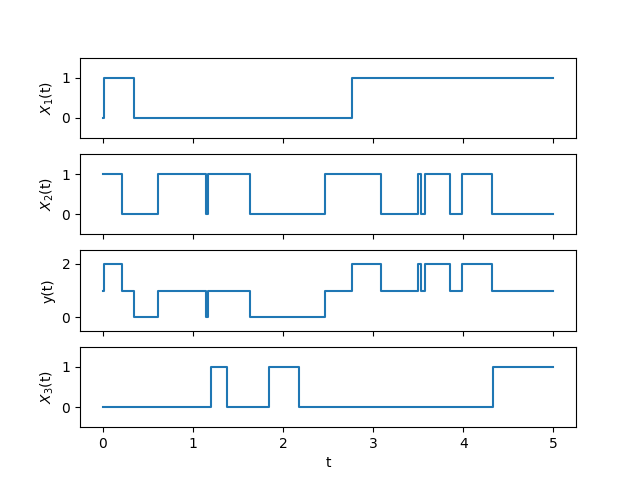
\includegraphics[width=.60\textwidth]{figures/traj}
		\caption{Sampled trajectories}
		\label{fig:simulation}
	\end{center}
\end{figure}
... illustrates the belief state trajectory given the observations. For the reference, the belief state update using particle filter and exact update is given together in ....... As can be seen from the figures, the exact update is well approximated by the particle filter.
\begin{figure}[H]
	\begin{center}
		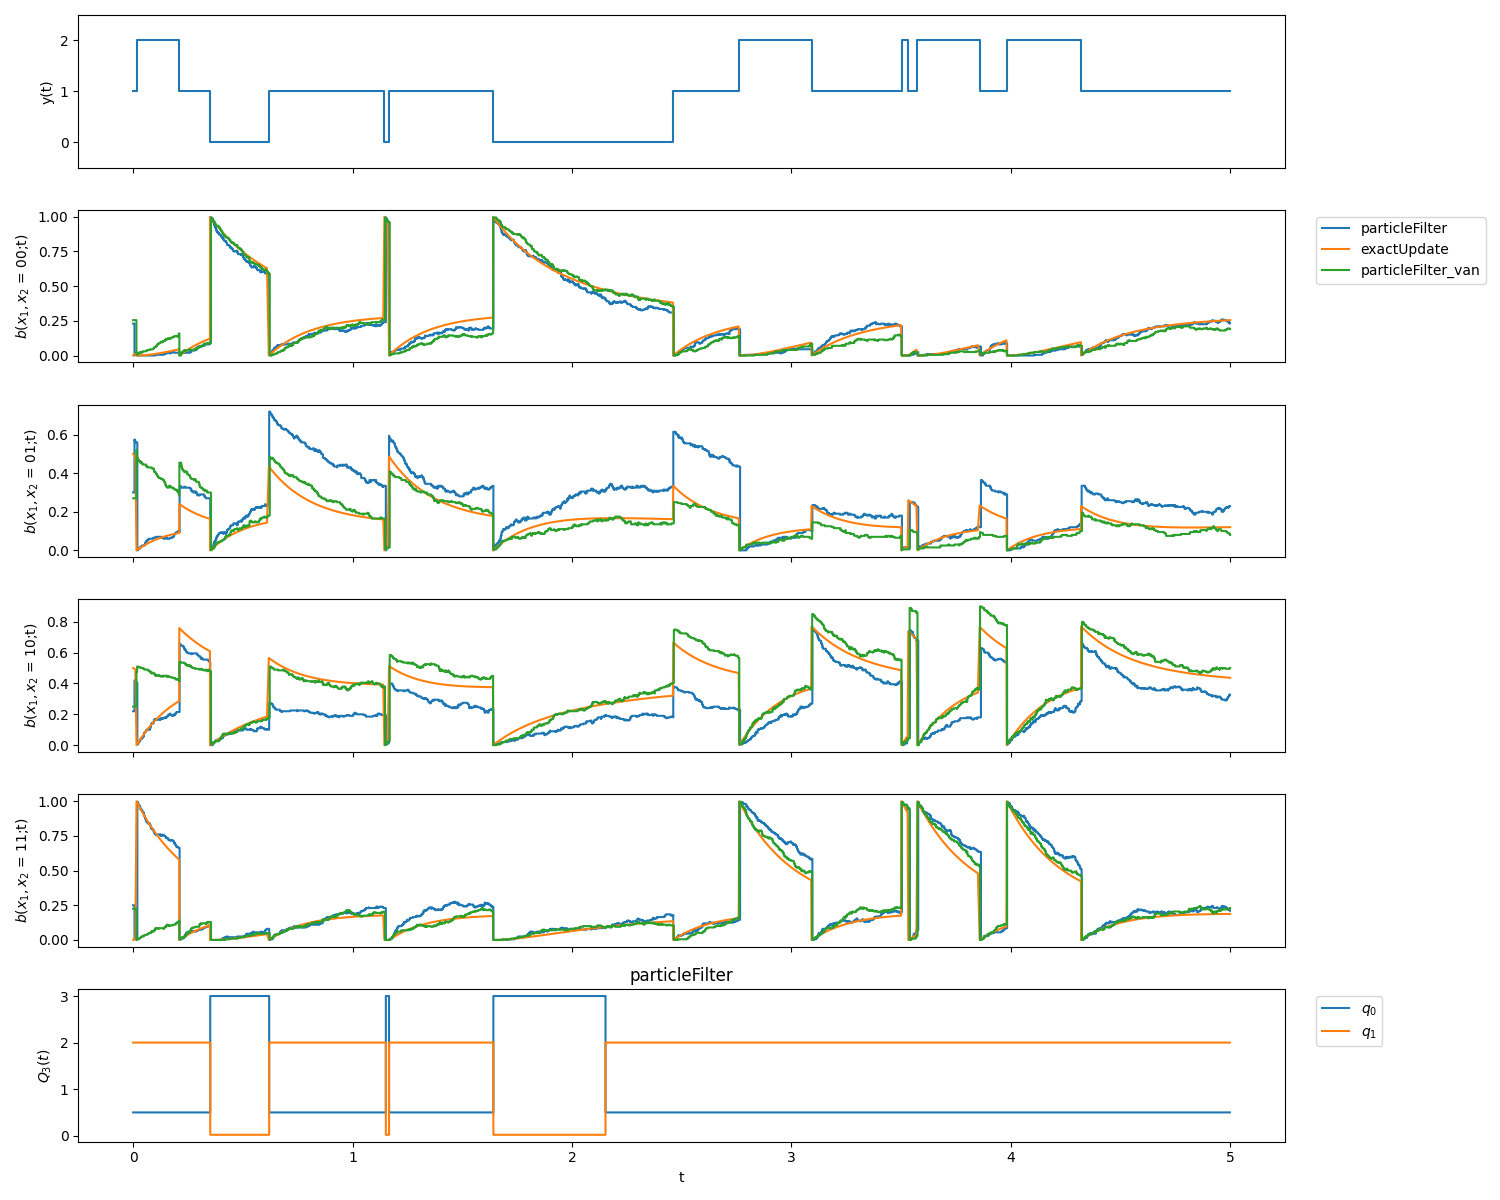
\includegraphics[width=.60\textwidth]{figures/b_q_traj}
		\caption{Belief state and $ Q_3 $ trajectories}
		\label{fig:b_q_traj}
	\end{center}
\end{figure}
Finally, the resulting $ Q_3 $ and trajectory of agent are given in ..... The trajectory shown in ...., are derived from the belief state update by particle filter which is given in .........
\begin{figure}[H]
	\begin{center}
		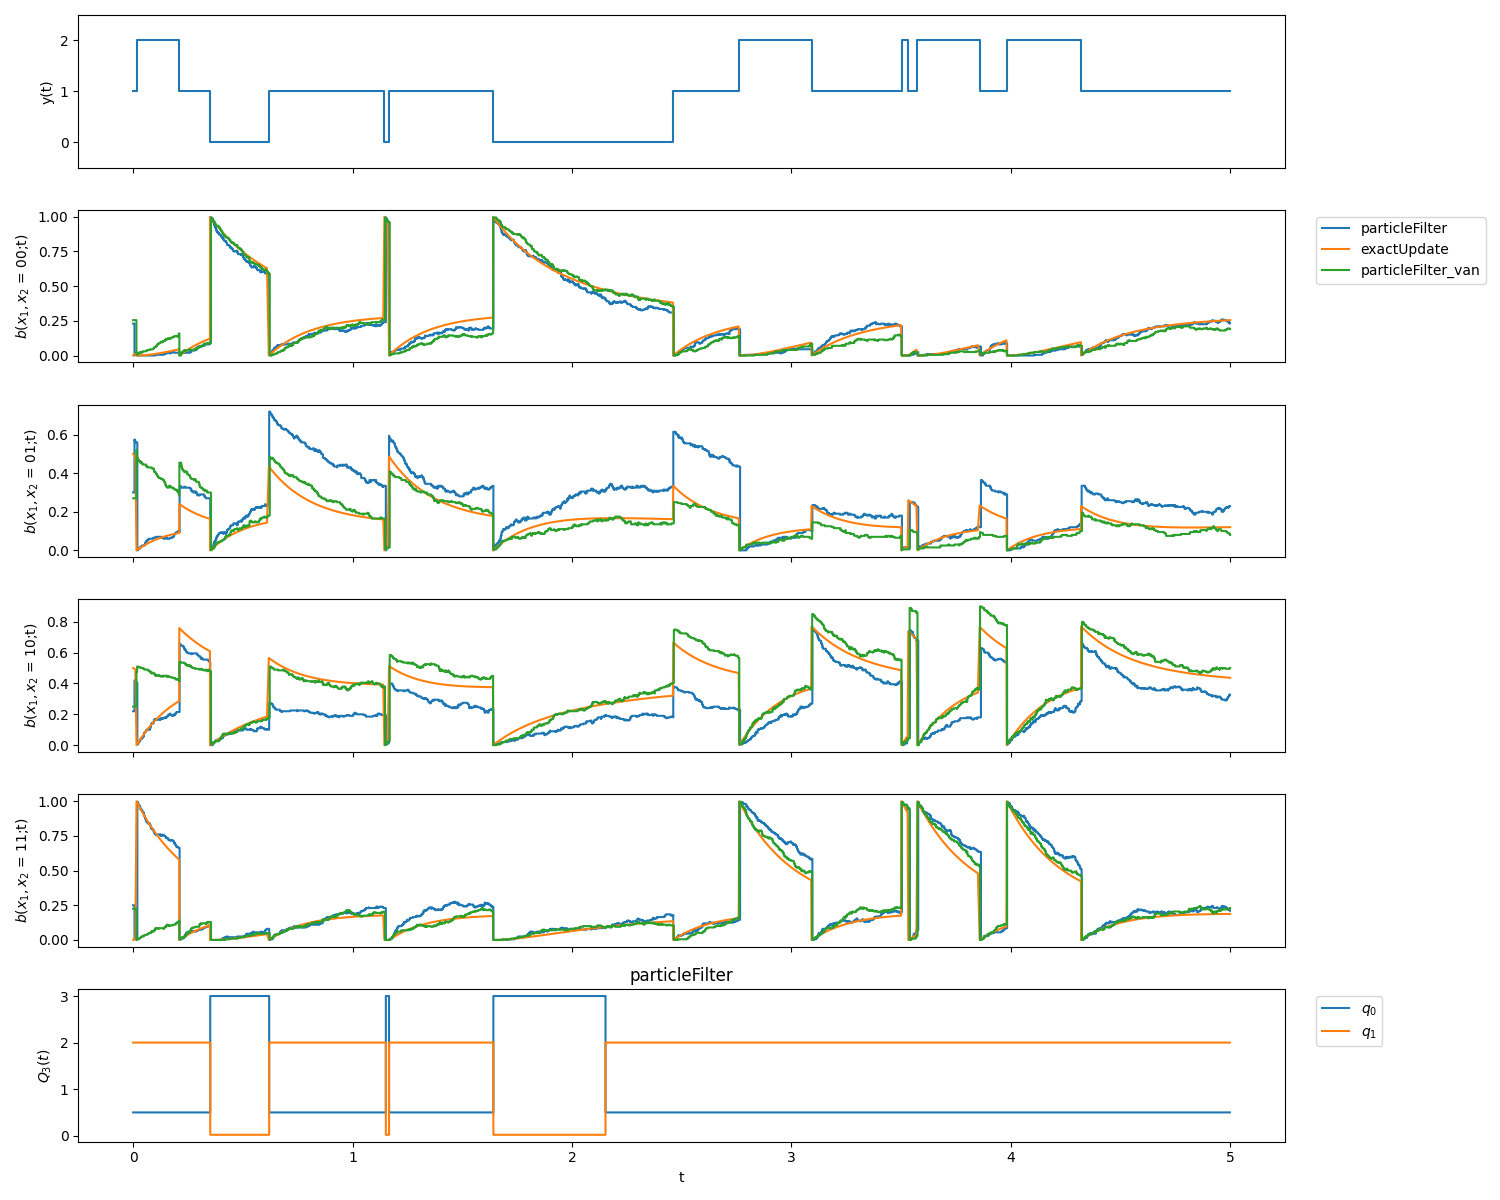
\includegraphics[width=.60\textwidth]{figures/b_q_traj}
		\caption{Belief state and $ Q_3 $ trajectories}
		\label{fig:b_q_traj}
	\end{center}
\end{figure}
\section{Inference of Observation Model}
\subsection{Equivalence Classes}
\label{sec:eq_classes}
As mentioned in \cref{sec:inf_setup}, the deterministic nature of the observation model results in a number of possible observation models. The setting described in \cref{chap:3} with configurations given in \cref{sec:config} leads to 81 observation models. However, with this experimental setup and the methods, it is only possible to distinguish these observation models into 10 different classes. Due to this equivalence, the inference problem is considered only for 10 observation models, each one representing one class. The reasons of this phenomena are discussed in detail in \cref{ap:eq_classes}, together with the observation models considered in inference problem. \\
\autoref{fig:llh_exactUpdate_81model} illustrates this situation clearly. The plot depicts the results of an experiment with 200 samples, $ |\xi_T| = 200 $, simulated using parameters $ \theta $, and the average likelihood of samples calculated for all 81 observation models. Here, the belief state is updated using exact method as described in \cref{par:bs_exact}, in order to depict the exact equivalence within one class. As can be seen, the results separate the set of observation models into 10 distinct classes.
\begin{figure}[H]
	\begin{center}
		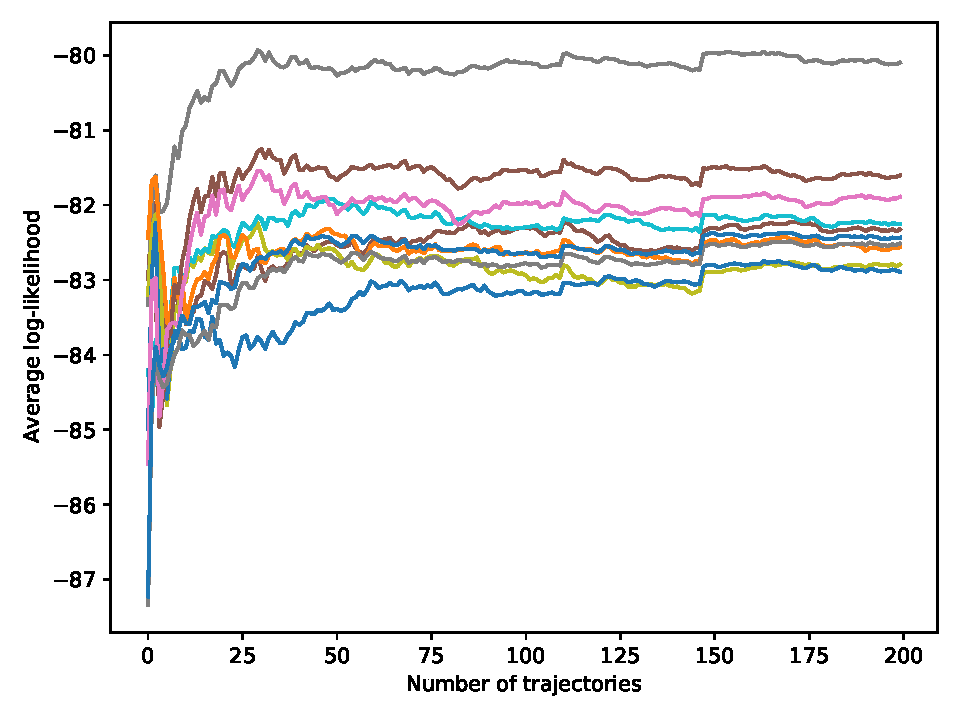
\includegraphics[width=.60\textwidth]{figures/equivalence_classes/llh_exactUpdate_81model}
		\caption{Belief state and $ Q_3 $ trajectories}
		\label{fig:llh_exactUpdate_81model}
	\end{center}
\end{figure}
In order to show the validity of the classes in the case of particle filter, the likelihood results from the observation models in the same class are given in ..... As can be seen from the graph, the observation models lead to so similar results to each other that they are assumed to be identical. 

\begin{figure}[H]
	\begin{center}
		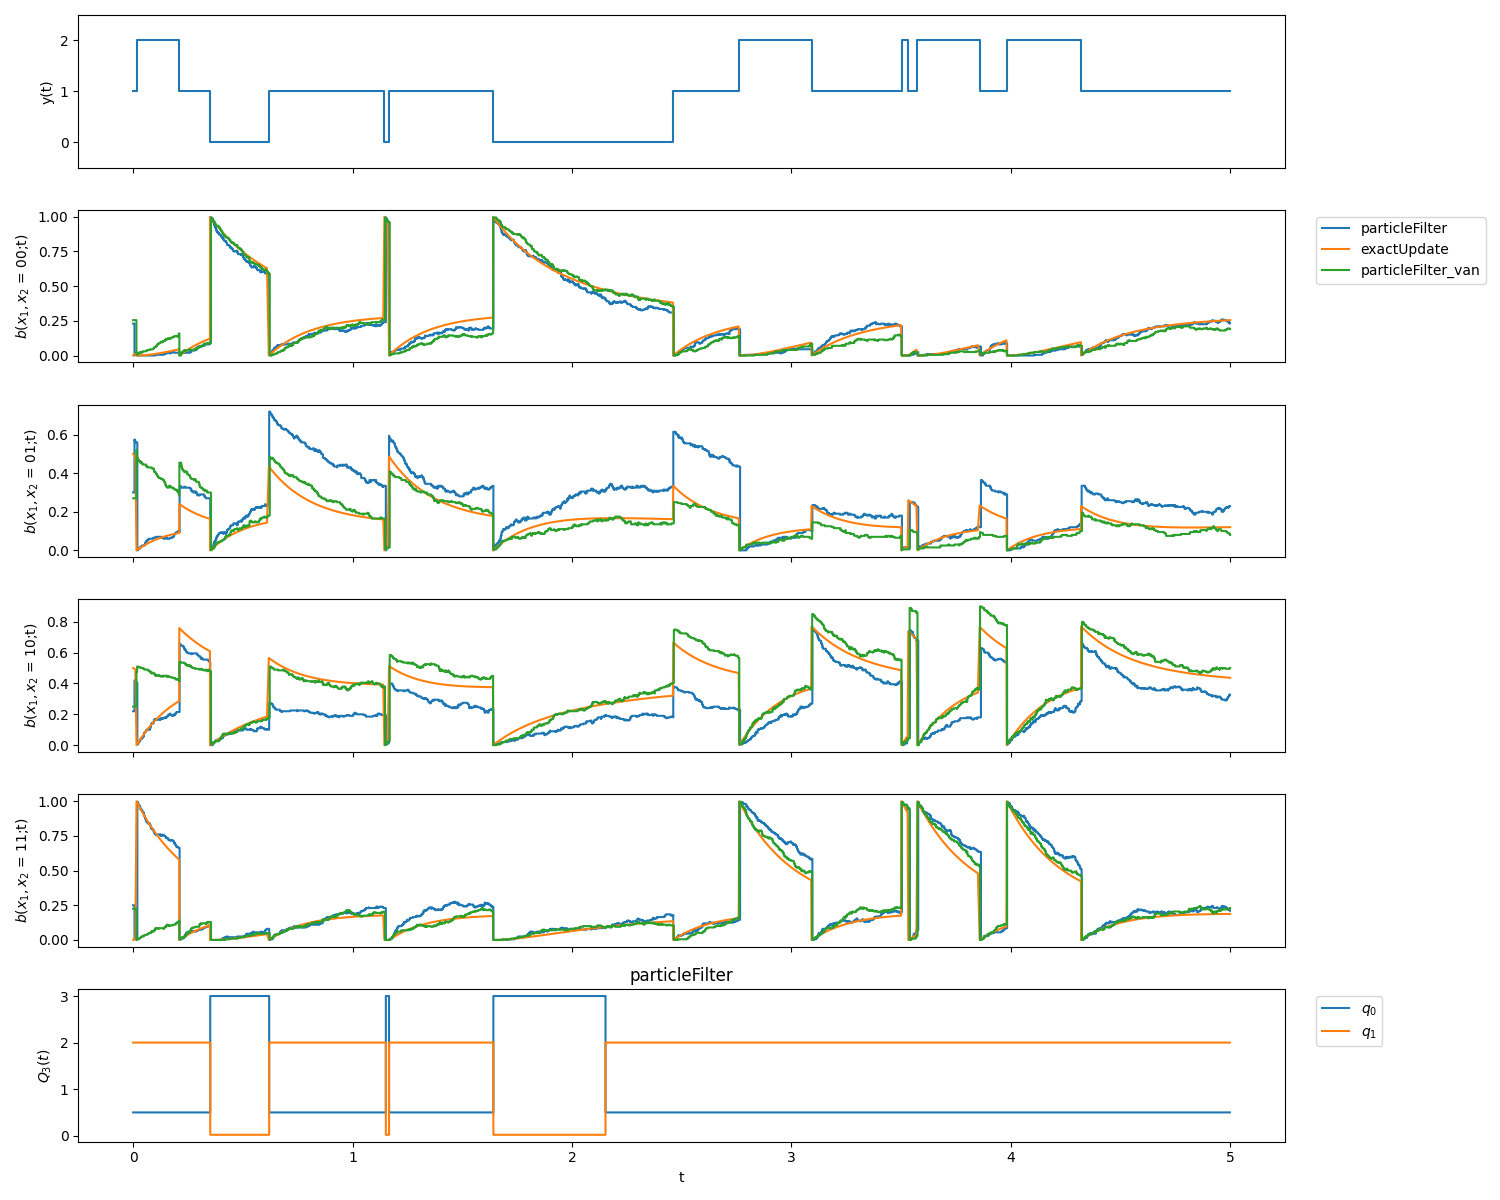
\includegraphics[width=.60\textwidth]{figures/b_q_traj}
		\caption{Belief state and $ Q_3 $ trajectories}
		\label{fig:b_q_traj}
	\end{center}
\end{figure}

%\subsection{Maximum Likelihood Estimation}
%\subsubsection{Equivalence Classes}
%
%$\psi_{true} =
%\begin{bmatrix} \vspace{-2pt}
%	1 & 0 & 0 \\  \vspace{-2pt}
%	0 & 1 & 0 \\  \vspace{-2pt}
%	0 & 1 & 0 \\  \vspace{-1pt}
%	0 & 0 & 1
%\end{bmatrix}$
%$\psi_{0} =
%\begin{bmatrix} \vspace{-2pt}
%1 & 0 & 0 \\  \vspace{-2pt}
%0 & 1 & 0 \\  \vspace{-2pt}
%0 & 1 & 0 \\  \vspace{-1pt}
%0 & 0 & 1
%\end{bmatrix}, 
%\psi_{1} =
%\begin{bmatrix} \vspace{-2pt}
%0 & 0 & 1 \\  \vspace{-2pt}
%0 & 1 & 0 \\  \vspace{-2pt}
%1 & 0 & 0 \\  \vspace{-1pt}
%0 & 0 & 1 
%\end{bmatrix},
%\psi_{2} =
%\begin{bmatrix} \vspace{-2pt}
%0 & 0 & 1 \\  \vspace{-2pt}
%1 & 0 & 0 \\  \vspace{-2pt}
%0 & 0 & 1 \\  \vspace{-1pt}
%0 & 1 & 0  
%\end{bmatrix}$
%
%\subsection{Maximum Likelihood Classification}
%\begin{figure}[htb]
%	\begin{subfigure}{.33\textwidth}
%		\centering
%		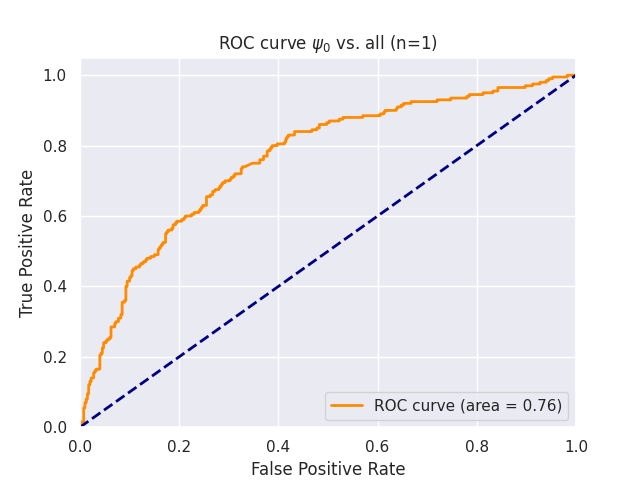
\includegraphics[width=1\linewidth]{figures/AUROC_600samples_class0_llh_n1}
%		\caption{}
%		\label{fig:sfig1}
%	\end{subfigure}%
%	\begin{subfigure}{.33\textwidth}
%		\centering
%		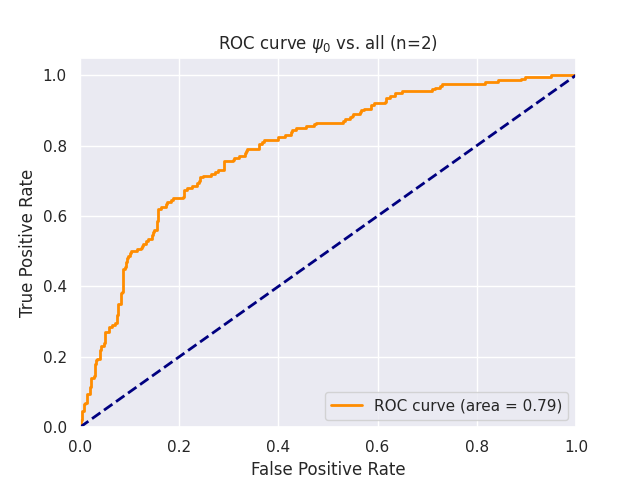
\includegraphics[width=1\linewidth]{figures/AUROC_600samples_class0_llh_n2}
%		\caption{}
%		\label{fig:sfig2}
%	\end{subfigure}
%	\begin{subfigure}{.33\textwidth}
%		\centering
%		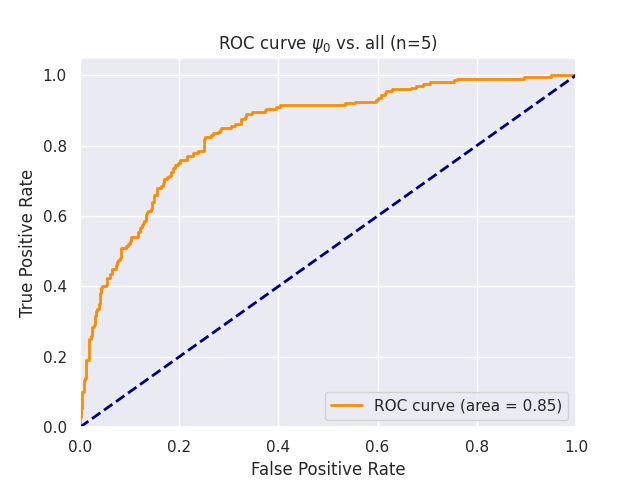
\includegraphics[width=1\linewidth]{figures/AUROC_600samples_class0_llh_n5}
%		\caption{}
%		\label{fig:sfig2}
%	\end{subfigure}\\
%	\begin{subfigure}{.33\textwidth}
%		\centering
%		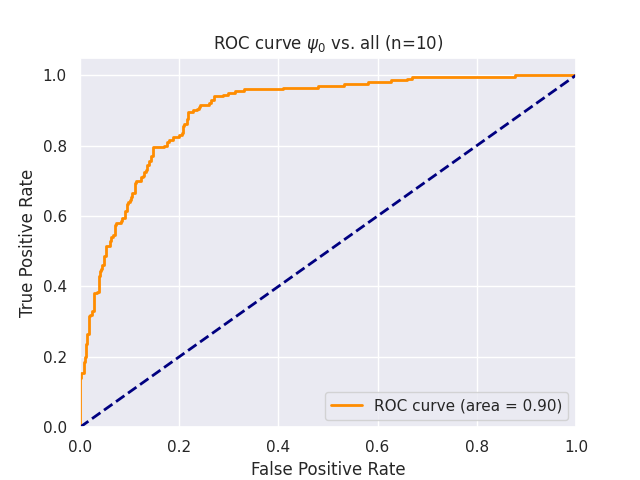
\includegraphics[width=1\linewidth]{figures/AUROC_600samples_class0_llh_n10}
%		\caption{}
%		\label{fig:sfig1}
%	\end{subfigure}%
%	\begin{subfigure}{.33\textwidth}
%		\centering
%		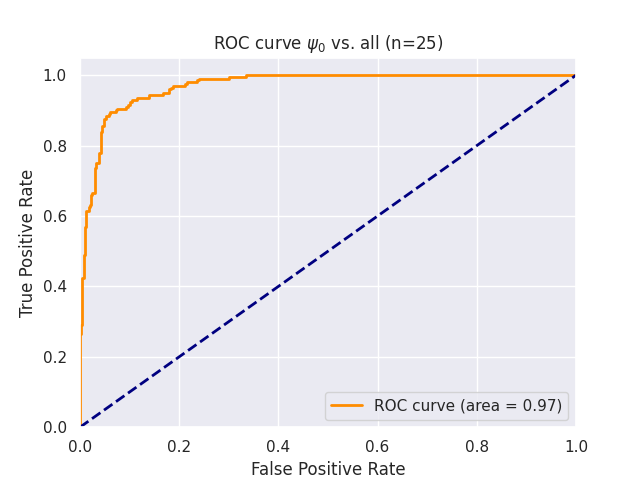
\includegraphics[width=1\linewidth]{figures/AUROC_600samples_class0_llh_n25}
%		\caption{}
%		\label{fig:sfig2}
%	\end{subfigure}
%	\begin{subfigure}{.33\textwidth}
%		\centering
%		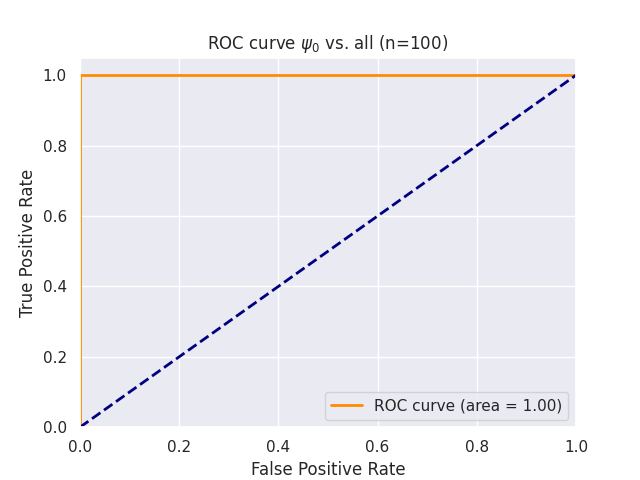
\includegraphics[width=1\linewidth]{figures/AUROC_600samples_class0_llh_n100}
%		\caption{}
%		\label{fig:sfig2}
%	\end{subfigure}
%	\caption{plots of....}
%	\label{fig:fig}
%\end{figure}
%\begin{figure}[htb]
%	\begin{center}
%		\includegraphics[width=.9\textwidth]{figures/all_particlefilter}
%		\caption{plot of...}
%		\label{fig:traj_}
%	\end{center}
%\end{figure}
